% !TeX root = chapter_classificationMethods.Rnw

\documentclass[tikz]{standalone}
 
\usetikzlibrary{positioning}
\usetikzlibrary{calc}
 
\begin{document}
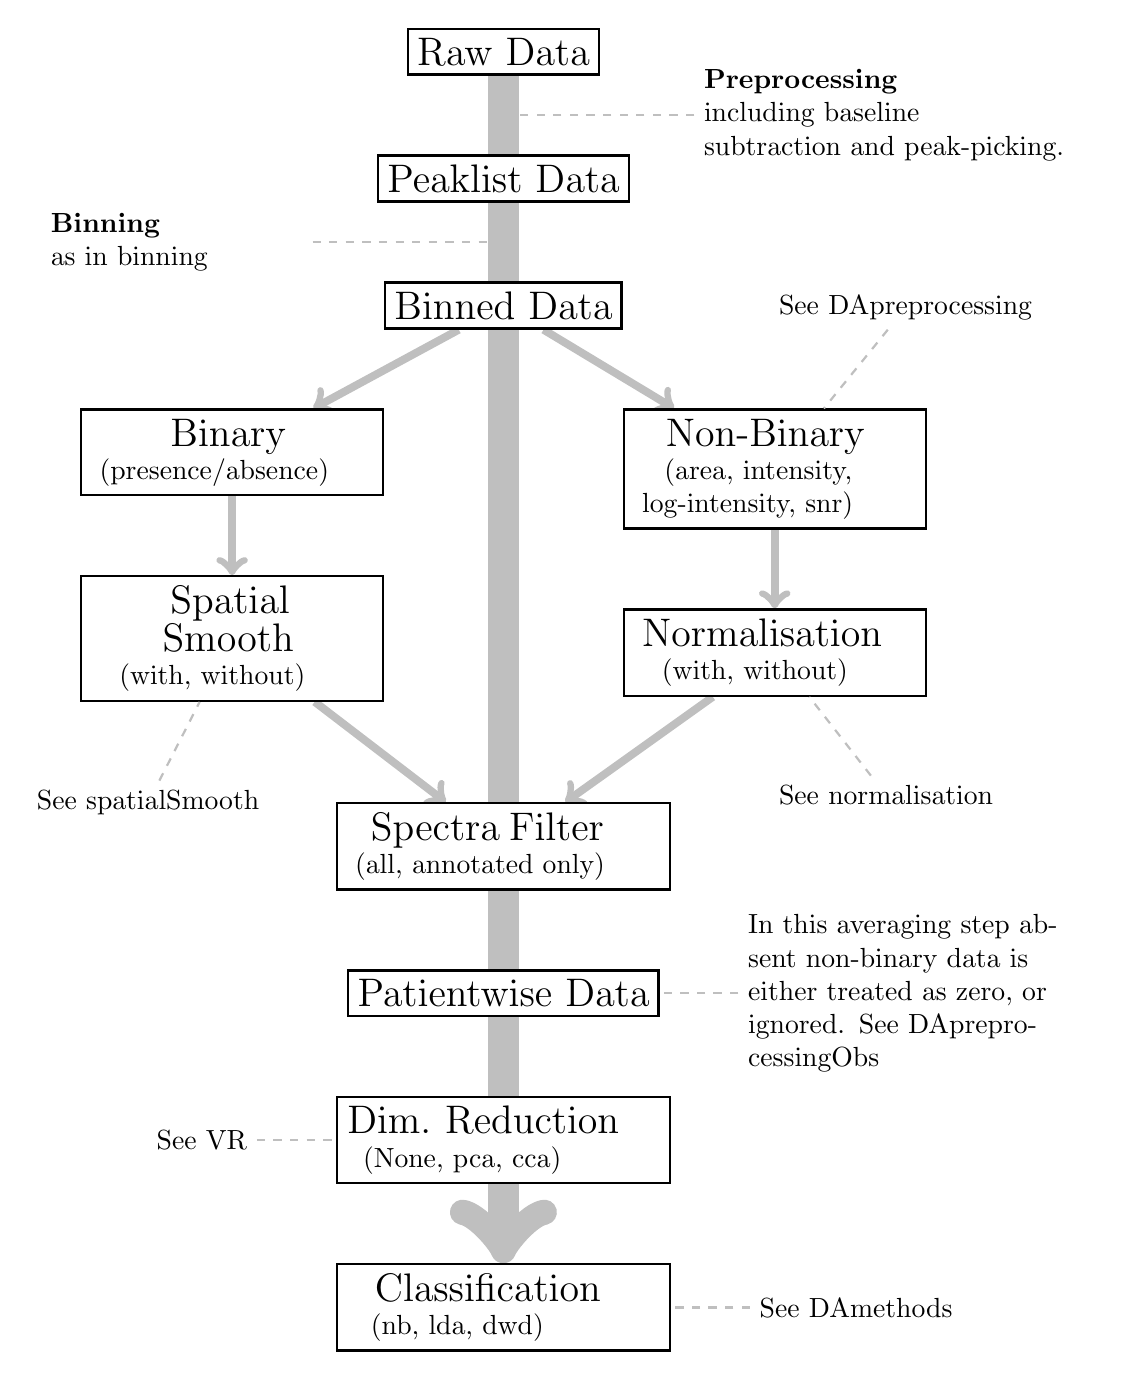
\begin{tikzpicture}

% \begin{scope}[on grid]

% \draw[help lines,step=5mm,gray!20] (5,-5) grid (17,12);





%%% Initialise Nodes
\draw (10,10) node[draw,thick] (a) {{\Large Raw Data }};
\node[draw,below=1cm of a,thick] (b1) {{\Large Peaklist Data}};
\node[draw,below=1cm of b1,thick] (b) {{\Large Binned Data}};
\node[draw,below left=1cm and 0cm of b, text width=3.6cm, thick] (c1) {{\Large \hspace{0.9cm} Binary } \\  \hspace{0cm} (presence/absence)};
\node[draw,below right=1cm and 0cm of b, text width=3.6cm, thick] (c2) {{\Large \hspace{0.3cm} Non-Binary } \\ \hspace{0.4cm}(area, intensity, \\ \hspace{0cm} log-intensity, \gls{snr})};
\node[draw,below=1cm of c1, text width=3.6cm, thick] (d1) {{\Large \hspace{0.9cm} Spatial \\ \hspace{0.8cm} Smooth } \\ \hspace{0.25cm} (with, without)};
\node[draw,below=1cm of c2, text width=3.6cm, thick] (d2) {{\Large \hspace{0cm} Normalisation } \\ \hspace{0.25cm} (with, without)};
\node[draw,below=6cm of b, text width=4cm, thick] (e) {{\Large \hspace{0.2cm} Spectra Filter } \\ \hspace{0cm} (all, annotated only)};
\node[draw,below=1cm of e,thick] (f) {{\Large Patientwise Data }};
\node[draw,below=1cm of f, text width=4cm,thick] (g) {{\Large \hspace{-0.1cm} Dim. Reduction } \\ \hspace{0.1cm} (None, \gls{pca}, \gls{cca})};
\node[draw,below=1cm of g, text width=4cm,thick] (h) {{\Large \hspace{0.25cm} Classification } \\ \hspace{0.2cm} (\gls{nb}, \gls{lda}, \gls{dwd})};

%%% Flow Lines
\draw[->, line width = 4mm, gray!50] (a) -- (h);
\draw[->, line width = 1mm, gray!50] (b) -- (c1);
\draw[->, line width = 1mm, gray!50] (b) -- (c2);
\draw[->, line width = 1mm, gray!50] (c1) -- (d1);
\draw[->, line width = 1mm, gray!50] (c2) -- (d2);
\draw[->, line width = 1mm, gray!50] (d1) -- (e);
\draw[->, line width = 1mm, gray!50] (d2) -- (e);

%%% Re-Initialise Nodes (draw over flow-lines)
\draw (10,10) node[draw, thick, fill=white] {{\Large Raw Data }};
\node[draw, below=1cm of a, thick, fill=white] {{\Large Peaklist Data}};
\node[draw, below=1cm of b1, thick, fill=white] {{\Large Binned Data}};
\node[draw, below left=1cm and 0cm of b, text width=3.6cm, thick, fill=white] {{\Large \hspace{0.9cm} Binary } \\  \hspace{0cm} (presence/absence)};
\node[draw, below right=1cm and 0cm of b, text width=3.6cm, thick, fill=white] {{\Large \hspace{0.3cm} Non-Binary } \\ \hspace{0.4cm}(area, intensity, \\ \hspace{0cm} log-intensity, \gls{snr})};
\node[draw, below=1cm of c1, text width=3.6cm, thick, fill=white] {{\Large \hspace{0.9cm} Spatial \\ \hspace{0.8cm} Smooth } \\ \hspace{0.25cm} (with, without)};
\node[draw, below=1cm of c2, text width=3.6cm, thick, fill=white] {{\Large \hspace{0cm} Normalisation } \\ \hspace{0.25cm} (with, without)};
\node[draw, below=6cm of b, text width=4cm, thick, fill=white] {{\Large \hspace{0.2cm} Spectra Filter } \\ \hspace{0cm} (all, annotated only)};
\node[draw, below=1cm of e, thick, fill=white] {{\Large Patientwise Data }};
\node[draw, below=1cm of f, text width=4cm, thick, fill=white] {{\Large \hspace{-0.1cm} Dim. Reduction } \\ \hspace{0.1cm} (None, \gls{pca}, \gls{cca})};
\node[draw, below=1cm of g, text width=4cm, thick, fill=white] {{\Large \hspace{0.25cm} Classification } \\ \hspace{0.2cm} (\gls{nb}, \gls{lda}, \gls{dwd})};



% %% Comments and Notes
\draw ($ (a) !.5! (b1) $) node (ab) {};
\node[right=2.3cm of ab,text width = 4.9cm] (s1) {{\bf Preprocessing } \\ including baseline \\ subtraction and peak-picking.};
\draw[dashed,gray!50,thick] (s1) -- (ab);

\draw ($ (b1) !.5! (b) $) node (bb) {};
\node[left=2.3cm of bb, text width = 3.2cm] (s2) {{\bf Binning } \\ as in \refapp{binning}};
\draw[dashed,gray!50,thick] (s2) -- (bb);

\node[above right=1cm and -2cm of c2] (s3) {See \refsec{DApreprocessing}};
\draw[dashed,gray!50,thick] (s3) -- (c2);

\node[below right=1cm and -2cm of d2] (s4) {See \refsec{normalisation}};
\draw[dashed,gray!50,thick] (s4) -- (d2);

\node[below left=1cm and -2.4cm of d1] (s5) {See \refsec{spatialSmooth}};
\draw[dashed,gray!50,thick] (s5) -- (d1);

\node[right=1cm of f, text width=4cm] (s6) {In this averaging step absent non-binary data is either treated as zero, or ignored. See \refsec{DApreprocessingObs}};
\draw[dashed,gray!50,thick] (s6) -- (f);

\node[left=1cm of g] (s7) {See \refsec{VR}};
\draw[dashed,gray!50,thick] (s7) -- (g);

\node[right=1cm of h] (s8) {See \refsec{DAmethods}};
\draw[dashed,gray!50,thick] (s8) -- (h);

% \draw ($ (e) !.5! (f) $) node (ef) {};
% \node[right=2.3cm of ef, text width = 4.9cm] (s6) {{\bf Smoothing } \\ as in ...};
% \draw[dashed,gray!50,thick] (s6) -- (ef);
% 
% \draw ($ (f) !.5! (g) $) node (fg) {};
% \node[left=2.8cm of fg, text width = 3.4cm] (s7) {{\bf Clustering } \\ as in ...};
% \draw[dashed,gray!50,thick] (s7) -- (fg);
% 
% \draw ($ (g) !.5! (h) $) node (gh) {};
% \node[right=2.3cm of gh, text width = 4.9cm] (s8) {{\bf DIPPS } \\ as in ...};
% \draw[dashed,gray!50,thick] (s8) -- (gh);
% 
% \draw ($ (h) !.4! (i) $) node (hi) {};
% \node[left=2.8cm of hi, text width = 3.4cm] (s9) {{\bf Jaccard Index } \\ as in ...};
% \draw[dashed,gray!50,thick] (s9) -- (hi);



% \end{scope}


\end{tikzpicture}
\end{document}


